\begin{figure}
	\centering
	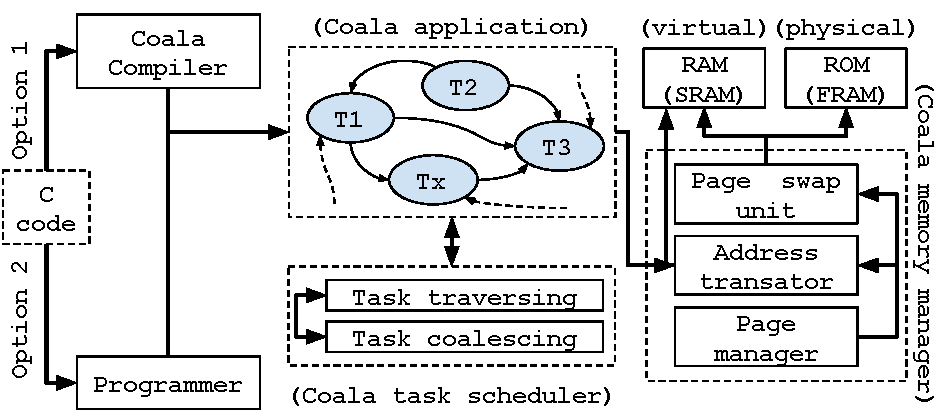
\includegraphics[width=\columnwidth]{figures/viper_block_diagram.pdf}
	\caption{\sys top-level view.}
	\label{fig:system_overview}
\end{figure}

\sys is a new programming and execution model for intermittent computing on energy-harvesting devices. \sys addresses the challenges motivated in Section~\ref{sec:background} to make task-based intermittent programs {\em efficient}, {\em flexible}, and {\em programmable}. \sys accomplishes this goal with a constellation of a new programming model, compiler, and run time software system support, refer to Figure~\ref{fig:system_overview}.

\noindent \textbf{\sys Programming Model:} To use \sys, a programmer first writes plain, imperative C code. The programmer then has an option to {\em manually} or {\em automatically} translate the program into code for \sys's task-based programming model. To manually translate, the programmer decomposes the program into tasks, and annotates memory accesses that manipulate data shared by multiple tasks. To automatically translate, the programmer simply uses \sys's compiler (described in Section~\ref{sec:compiler}), which decomposes a program into tasks and annotates accesses to task-shared data. After translating to task-based code and compiling, the programmer has an executable \sys binary.

\sys consists of its compiler and the run time software support for its execution model and includes several lightweight programming model extensions similar to those in prior work~\cite{chain,alpaca}. Table~\ref{tab:viper_syntax} provides an overview of these extensions, which can be used manually by a programmer or added to a program automatically, using \sys's compiler. As in prior task-based intermittent programming models~\cite{chain,alpaca}, a \sys program is decomposed into tasks, which are functions that are not allowed to have any direct callers. The programmer identifies a task by adding the {\tt task} keyword to the function's declaration. A programmer invokes one task, {\tt t} from another task {\tt u} using {\tt next\_task( t )}, which atomically commits the state of {\tt u} and transfers control to the entry point of {\tt t}. A program has a single {\em origin} task that executes first during the program's first execution; after a power failure, in subsequent operating periods, \sys restarts from the task that was executing just before the failure.

A \sys program manipulates {\em protected} state---accessed by more than one task---using the {\tt RP} and {\tt WP} operations, which read and write (respectively) a protected variable. These operations convey to \sys's runtime system which data must be protected through paging by the memory manager.   

\begin{table}
	\centering
	\footnotesize
	\begin{tabular}{|c|c|}
		\hline
		Keyword & Description\\
		\hline\hline
		\texttt{task foo(){...}} & Task declaration\\
		\texttt{origin task foo(){...}} & Origin task declaration\\
		\texttt{next\_task()} & Transition to a new task\\
		\texttt{RP} & Read-protected variable\\
		\texttt{WP} & Write-protected variable\\
		\hline
	\end{tabular}
	\caption{Summary of \sys's programming model extensions}
	\label{tab:viper_syntax}
\end{table}

\noindent \textbf{\sys Memory Manager:} When the binary executes, \sys's runtime support affects its execution through {\em (virtualizing) memory manager} (described in Section~\ref{sec:memory_virtulaization}) and {\em (coalescing) task scheduler} (described in Section~\ref{sec:task_coalescing}). The \sys binary executes its tasks correctly, with consistent memory state, due to \sys's virtual memory mechanism. Relying on programmer or compiler annotation of accesses to memory locations that might be shared between tasks, \sys's memory virtualization {\em pages} these data to SRAM from FRAM as they are needed. Tasks operate, accessing SRAM only, demand-paging data to accommodate a SRAM smaller than FRAM\todo{Sentence unclear}{Brandon}. When a task completes, \sys commits modified, paged data back to its original FRAM location atomically ensuring subsequent tasks page in correct memory state. 

\noindent \textbf{\sys Task Scheduler:} \sys runs a lightweight task scheduler that uses {\em task coalescing} to make \sys's statically defined tasks efficiently use available energy. By default, tasks run in sequence and each task commits as it completes, potentially incurring unnecessary overhead for commits between consecutive, non-failing tasks. \sys dynamically coalesces consecutive tasks by deferring the commit of an earlier task until the completion of a later task. \sys's memory management mechanism facilitates coalescing because \sys can defer an earlier task's commit by simply buffering modified, paged data as the later task executes. After coalescing a sequence of tasks, \sys commits all tasks' updates to FRAM, together, combining tasks updates to the same pages and minimizing the commit overhead.